\documentclass[11pt]{article}
\usepackage[margin=1in]{geometry}
\usepackage{amsmath,amssymb}
\usepackage{graphicx}
\usepackage[super,comma,sort&compress]{natbib}
\usepackage{booktabs}
\usepackage{hyperref}
\usepackage{xcolor}
\usepackage{lineno}
\graphicspath{{../figures/}}
\setlength{\emergencystretch}{2em}

\title{Stationary-measure correction for force-free molecular dynamics via a
mode-resolved generalized Langevin readout}
\author{[Author list and affiliations to be supplied]}
\date{}

\begin{document}
\maketitle

\begin{abstract}
Force-free direct propagators can accelerate molecular dynamics by large factors, but their
long-time equilibrium statistics are unreliable. We show that pointwise one-step accuracy is
neither necessary nor sufficient for long-time fidelity: a published propagator with a large
pointwise error reproduces the canonical water ensemble, while a pointwise-accurate model fails.
The failure is a mode-resolved stationary-measure problem, not an NVE energy problem. We
introduce a fixed mode-resolved generalized Langevin readout (GLR): a frozen propagator supplies
the displacement, while per-mode AR($p$) memory kernels fitted from the reference velocity
autocorrelation and exact group-resolved variance rescaling enforce the canonical mean kinetic
partition by construction, with a stochastic target that restores the kinetic-energy marginal
(Gamma-distributed); the joint position--velocity distribution is not guaranteed. The
readout algorithm is fixed; the backbone and the physics-defined mode basis are the only plug-ins.
On water, the GLR matches multi-lag velocity
correlations, and is stable and initial-condition independent. Applied to two different frozen
backbones---a relational propagator and a phase-space operator---it makes both stable and
canonically partitioned; in a covalent solid with a 5 fs backbone, a stochastic phonon-band
variance rescale restores the canonical kinetic-energy variance, enforces Si/O equipartition,
improves the Si--O RDF, and preserves the phonon VDOS. At
100 ps, it improves the
O--H RDF from 0.118 to 0.104 and the O VDOS from 0.937 to 0.964 over the published checkpoint; at
2.5 ns the O--H RDF reaches 0.038. It yields a diffusion coefficient of
1.39--1.41 $\times 10^{-9}$ m$^2$ s$^{-1}$ on two starts,
within 26\% of the reference 1.84--1.88 $\times 10^{-9}$ m$^2$ s$^{-1}$ and far closer than the
AR(1) readout (3.59 $\times 10^{-9}$). The readout is training-free, force-free, and applicable
to other frozen propagators in principle.
\end{abstract}

\section{Introduction}

Molecular dynamics (MD) is the workhorse for connecting microscopic interactions to the
macroscopic behaviour of liquids, solids, and biological assemblies. Its central limitation is
time: the 1--2 fs integration step required for stable dynamics restricts routine simulations to
nanoseconds, while many phenomena of interest---diffusion, nucleation, conformational transitions,
and slow relaxation---unfold over microseconds to milliseconds. Machine-learned interatomic
potentials have reduced the cost of the force evaluation, but they retain the sequential
integrator and therefore the same step-count bottleneck.

A more radical route is to learn the propagator itself. Instead of evaluating forces and
integrating Newton's equations, a direct propagator maps a state at time \(t\) to a state at
\(t+\Delta t\) with \(\Delta t\) several times the stable integration step. Because the map is
force-free, it can in principle be evaluated at a fraction of the cost of an MD step and can be
rolled out autoregressively. TrajCast demonstrated that this idea is viable for liquid water: an
equivariant message-passing network trained on 5 fs pairs reproduces the oxygen--oxygen radial
distribution function (RDF), the vibrational density of states (VDOS), and the diffusion
coefficient under a global thermostat \cite{trajcast}. The result is an important existence proof:
faithful long-time water physics is possible without forces.

What the existence proof does not provide is a guarantee. A direct propagator is trained on
one-step pairs, usually by minimizing a displacement or velocity error. The quantity that matters
at long times, however, is the stationary measure of the composed map---the distribution of
positions and velocities that the autoregressive rollout visits after transients have decayed.
One-step accuracy constrains a conditional mean; it says little about the invariant measure of a
nonlinear, stochastic, or thermostatted iteration. The gap is familiar in spirit from generative
modelling, where a low reconstruction error does not imply a correct sample distribution, but it
has not been diagnosed systematically for force-free MD propagators.

Here we show that the gap is real and that it has a specific structure. Using water as a test
system, we compare a published TrajCast checkpoint with our own direct propagator. The published
model has a one-step position error about fifteen times larger than ours on held-out transitions,
yet it reproduces the canonical mode partition, RDF, and VDOS, whereas our pointwise-better model
develops a large mode imbalance and fails the same 100 ps NVT screen. The ranking by one-step
error is therefore not just noisy---it can be inverted. A second diagnostic removes another
plausible explanation: 25 ps NVE energy drift does not order the models either. The published
model heats strongly in NVE and still passes NVT; our most NVE-stable model fails NVT. The
relevant object is the composed propagator plus thermostat, and the relevant failure is a bias in
the mode-resolved stationary measure, not a one-step error or an energy-integration error. This
is an existence proof from two models, not a controlled correlation: the checkpoints differ in
architecture and training data, so the inversion establishes that one-step accuracy is neither
necessary nor sufficient, not that it is generally anti-correlated with ensemble fidelity.

Existing remedies attack different parts of this problem. Global stochastic thermostats, such as
CSVR, control the total kinetic energy but not its distribution among molecular translation,
rotation, and internal motion \cite{csvr}. Structure-preserving learned maps enforce symplectic or
time-reversible structure and improve energy conservation and equipartition \cite{bigi_action},
but they are deterministic and target mechanical structure rather than the canonical NVT measure.
Learned velocity updates recover stability by injecting an LSTM prediction periodically
\cite{mamd}, but the update is a black box and is not tied to the equilibrium mode partition.
Generalized Langevin equation (GLE) thermostats provide memory kernels and colored noise with the
correct fluctuation--dissipation relation \cite{ceriotti_prl,ceriotti_jctc}, and
frequency-resolved thermostats can control selected modes \cite{zpe_thermostat}, but these are
thermostats for an MD integrator, not readouts for a frozen force-free propagator. Stochastic and
generative propagators offer another route---Timewarp accelerates dynamics with learned
time-coarsening \cite{timewarp}, and generative models such as MDGen sample trajectory
distributions \cite{mdgen}---at the cost of MCMC, an energy function, or a substantially larger
generative model.

We take a different decomposition. A frozen force-free backbone is responsible for structure: it
supplies the displacement \(\Delta q_t\). A lightweight, mode-resolved generalized-Langevin
readout (GLR) is responsible for thermodynamics: it supplies the velocity that enters the next
backbone call and the kinetic diagnostics. The readout decomposes the velocity into molecular
translation, rotation, and internal modes; fits a per-mode AR(\(p\)) memory kernel to the
reference velocity autocorrelation by Yule--Walker; injects fluctuation--dissipation-consistent
noise with the prediction-error variance; and rescales each mode or group to its canonical kinetic-energy target
energy \(N_a k_B T/2\) at every step. The partition is therefore enforced by construction, while
the memory kernel matches the multi-lag dynamics that a single gain cannot capture. The backbone
is not retrained, and the readout is fitted from a short reference NVT trajectory.

We apply the GLR to SPC/Fw water \cite{spcfw} and compare it with the published TrajCast
checkpoint, our 250k direct propagator, an AR(1) readout, and several negative controls. The GLR
is stable for 100 ps from two independent initial conditions, is initial-condition independent in
its partition, ACF, RDF, and VDOS, and reproduces the O--O, O--H, and H--H RDFs and the O VDOS
more closely than the published checkpoint in our analysis. The 2.5 ns production run tests the
diffusion coefficient---the last long-time observable---and the ablations isolate the roles of
the memory order, the FD noise, the variance rescale, and the displacement coupling. The result is
a practical route, demonstrated here on water, for making a force-free propagator
thermodynamically consistent without retraining it, and a diagnostic that explains when and why
such a propagator will fail.

\subsection*{Contributions}

\begin{enumerate}
\item A diagnostic showing that pointwise one-step accuracy is neither necessary nor sufficient
  for long-time equilibrium, and that NVE energy stability is not the discriminating variable.
\item Evidence that the failure is a mode-resolved stationary-measure bias of the composed
  propagator plus thermostat.
\item A mode-resolved AR(\(p\)) FD readout with exact group-resolved variance rescaling that
  guarantees the canonical mean kinetic partition (and the marginal with the stochastic target)
  and matches multi-lag mode ACFs on a frozen force-free
  propagator.
\item Water results at or beyond the published TrajCast checkpoint on RDF and VDOS, with diffusion
  and initial-condition independence tested at 2.5 ns, plus ablations that isolate each component.
\end{enumerate}

\section{Results}

\subsection{Pointwise accuracy does not order long-time fidelity}

We first asked whether the conventional training objective---one-step displacement or velocity
error on held-out transitions---predicts the long-time behaviour of a force-free propagator. We
compared two models trained on the same SPC/Fw water data: our 250k relational propagator and the
published TrajCast water checkpoint. On 1,250 held-out transitions, the published checkpoint has a
mean absolute position error of \(4.75\times10^{-3}\) \AA{} and a velocity error of
\(1.63\times10^{-3}\) \AA{} fs\(^{-1}\). The 250k model is about fifteen times more accurate
pointwise (\(2.97\times10^{-4}\) \AA{} and \(1.09\times10^{-4}\) \AA{} fs\(^{-1}\)). If one-step
accuracy controlled long-time fidelity, the 250k model should be the better sampler.

It is not. Under the same 100 ps NVT protocol (300 K, CSVR, 5 fs), the published checkpoint
reproduces the canonical kinetic partition---translation \(2.505\) eV, rotation \(2.463\) eV,
internal \(2.444\) eV against the 2.5 ns reference means of \(2.459\), \(2.502\), and \(2.450\)
eV (the first 100 ps reference block is an outlier at \(2.373/2.430/2.609\) eV)---and gives
O--O, O--H, and H--H RDF RMSEs of 0.043, 0.118, and 0.096. The 250k model, despite its lower
one-step error, collapses the collective modes and overheats the internal mode: translation
\(0.538\) eV, rotation \(0.786\) eV, internal \(6.044\) eV. Its RDF RMSEs are 0.646, 1.312, and
0.249. The total kinetic energy is close to the target in both cases; the distribution across
modes is not. A pointwise-better model is a worse sampler, and the failure is invisible to the
training loss.

The inversion is not a peculiarity of one checkpoint. A 20k-step prefix of the same architecture
is even more pointwise accurate but becomes unstable in NVT after about 50 ps. A native TrajCast
architecture trained to only about 10\% of its schedule has a pointwise error three times smaller
than the 250k model and fails in the opposite direction---translation \(3.256\) eV, rotation
\(3.105\) eV, internal \(1.041\) eV. The sign of the mode bias is architecture- and
training-dependent, but its presence is not.

\subsection{NVE energy drift is a red herring}

A natural second hypothesis is that the failing models inject energy and heat, and that a better
energy integrator would fix the ensemble. We tested this directly with 25 ps NVE rollouts from the
same initial state. The published checkpoint heats from 302 K to 476 K; the 250k model cools from
302 K to 271 K; the NVT-pair fine-tuned M0 model heats to 387 K. The ordering by NVE drift is
essentially the reverse of the ordering by NVT fidelity: the model that heats the most passes the
NVT screen, and the most NVE-stable model fails it. Energy conservation and canonical sampling are
different properties of the composed map. A force-free propagator can be a poor energy integrator
and a good thermostat, or vice versa; NVE drift cannot be used as a surrogate for the stationary
measure.

\subsection{The failure is a mode-resolved partition bias}

The two diagnostics point to a common variable: the distribution of kinetic energy among molecular
modes. Figure~\ref{fig:diagnostic}c shows the mode kinetic energy relative to the reference for all
models. The failing models are not simply hot or cold. They are partitioned: the 250k family is
collectively cold and internally hot (translation 0.23, rotation 0.32, internal 2.32 of the
reference), the native/M0 family is collectively hot and internally cold (1.37, 1.28, 0.40), and
the published checkpoint is close to the reference on all three (1.06, 1.01, 0.94). The total
temperature is approximately 300 K in every case. A global thermostat holds the scalar temperature
while leaving the vector of mode temperatures biased.

This resolves the apparent paradox. The one-step loss is dominated by the conditional mean of the
displacement, which is insensitive to a slow redistribution of kinetic energy across modes. The
NVE trajectory measures the total energy budget, which can drift without changing the mode
partition in the same way. The NVT stationary measure is the object that sees the bias, and the
mode partition is its most informative low-dimensional projection.

\subsection{Stability is not correctness}

The distinction matters because long rollouts are often used as the acceptance test.
Figure~\ref{fig:diagnostic}d plots the longest stable NVT run against the partition verdict. The
phase-space v0 model is stable for 2.75 ns and has a partition of 0.111/0.808/6.338 eV; the 250k
and Current-Only models are stable for 150 ps with the same bias. Stability without partition
correctness is a long-lived wrong answer, not a success. Conversely, short-horizon fixes can
destabilize: the M0 endpoint fine-tune passes on the val\_04 start but blows up at 130 ps on an
independent start, and the 5-step CSRV moment loss blows up at 4.3 ps. The acceptance criterion
must be the stationary measure, not the absence of a numerical crash.

These results define the design requirement for a remedy. The propagator must be paired with a
readout that controls the \emph{mode-resolved} kinetic partition and the \emph{multi-lag} dynamics,
not just the total temperature or a single-lag gain. The readout should not require retraining the
backbone, and it should be evaluated on the same long-time observables that expose the failure.
The next section introduces such a readout.

\begin{figure}[t]
  \centering
  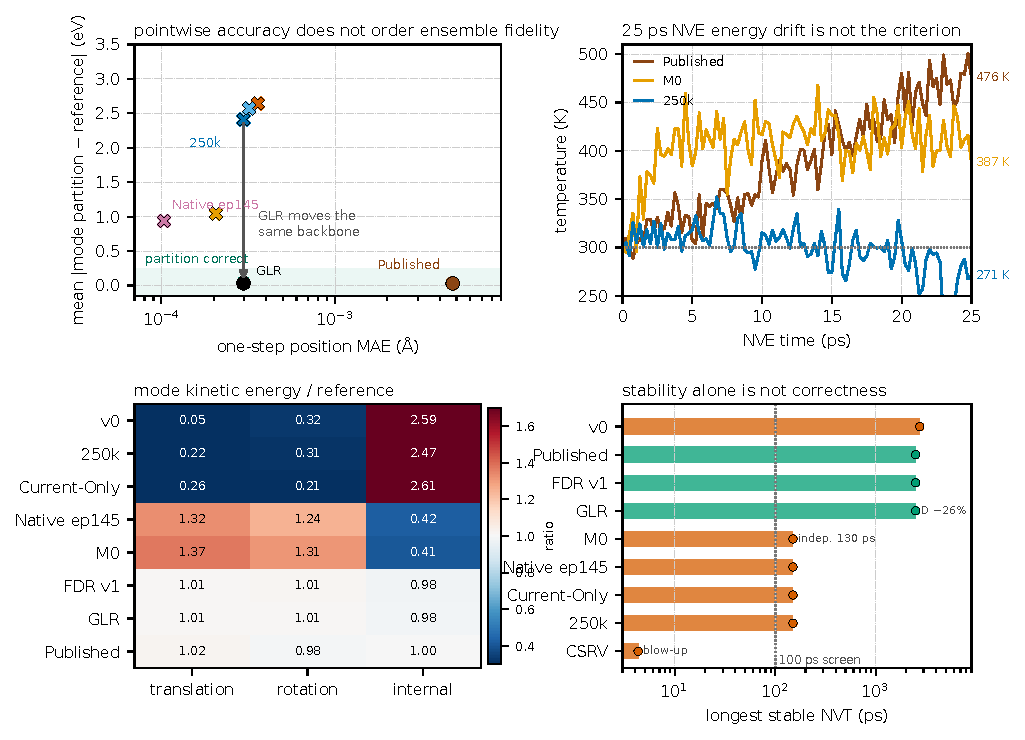
\includegraphics[width=\linewidth]{fig1_diagnostic.pdf}
  \caption{Pointwise accuracy and short-horizon stability do not predict NVT fidelity.
  (a) One-step position error versus mean absolute mode-partition error. The published checkpoint
  has a large one-step error but a correct partition; the 250k model is pointwise better and fails.
  The GLR moves the same 250k backbone to a correct partition without changing its position head.
  (b) 25 ps NVE temperature traces. (c) Mode kinetic energy relative to the reference NVT.
  (d) Longest stable NVT run and the partition verdict.}
  \label{fig:diagnostic}
\end{figure}

\subsection{A mode-resolved generalized Langevin readout}

\textbf{Framework.} The method has one fixed readout and two plug-ins: the frozen backbone
\(f_\theta\) and the physics-defined mode basis \(\mathcal M\). The readout algorithm is fixed:
(i) decompose the velocity into the modes in \(\mathcal M\); (ii) fit an AR(10) process to each
mode's reference ACF by Yule--Walker; (iii) add FD-consistent noise; (iv) blend with the backbone
velocity at \(\lambda=0.1\); (v) rescale each group to its canonical kinetic energy
(\(N_a k_BT/2\) in the deterministic limit, Gamma-distributed in the stochastic configuration);
(vi) project out the total centre-of-mass velocity. The position update is always
\(q_{t+1}=q_t+\Delta q_t\). The rest of the paper instantiates \(\mathcal M\) as molecular
translation/rotation/internal modes for water and as phonon bands for quartz, with a species
partition as a coarser control; the readout itself does not change. For quartz the memory kernel
is switched off because the 5 fs backbone already reproduces the phonon ACF; only the
variance-rescale component is active.

The diagnostic says that the missing object is a mode-resolved stationary measure. We therefore
leave the backbone unchanged and add a readout whose job is to enforce that measure. The
architecture is deliberately asymmetric. The frozen backbone supplies the displacement
\(\Delta q_t\); the readout supplies the velocity \(v_t\) that enters the next backbone call and
the kinetic diagnostics. The position update remains
\begin{equation}
q_{t+1}=q_t+\Delta q_t,
\end{equation}
so the learned displacement stays in distribution and the readout is not integrated as a second
position update. We tested the obvious alternative---adding the velocity correction to the
displacement---and it crashed at 24.8 ps (minimum interatomic distance 0.647 \AA), confirming that
the decoupling is a stability requirement rather than a stylistic choice.

The readout decomposes the velocity into molecular translation, rotation, and internal modes,
which are orthogonal under the mass-weighted inner product (Methods). For each mode, an AR(\(p\))
process is fitted to the reference velocity ACF by Yule--Walker; the prediction-error ratio
\(\rho_a\) sets the FD noise variance, \(\operatorname{Var}(\varepsilon^a)=\rho_a N_a k_BT/2\).
The AR prediction and the noise are blended with the backbone velocity,
\(v_t^{\rm blend}=(1-\lambda)v_t^{\rm pred}+\lambda\tilde v_t\) with \(\lambda=0.1\), and each mode
is rescaled to its canonical mean kinetic energy,
\begin{equation}
v_t^{\rm GLR}=\sum_a s_a\,(v_t^{\rm blend})^a,\qquad
s_a=\sqrt{\frac{N_a k_BT/2}{\tfrac12\sum_i m_i|(v_t^{\rm blend})_i^a|^2}}.
\end{equation}
The total centre-of-mass velocity is projected out after the rescale. The construction guarantees
the canonical mode/group kinetic-energy marginal (mean \(N_a k_BT/2\), Gamma-distributed in the stochastic configuration) at every step and the AR(\(p\)) stationary ACF up to lag
\(p\). The position marginal is not guaranteed analytically; it is learned by the backbone and
validated empirically. The per-step rescale suppresses the mode-KE fluctuations (reference std
about 0.24 eV versus about 0.002 eV), so the guarantee is on the first moment; the marginal
velocity distribution is nevertheless close to the reference (component kurtosis
2.93/5.49/5.93 versus 3.04/5.62/5.57 for translation, rotation, and internal motion). Throughout,
``thermodynamically consistent'' refers to this mean-partition-plus-ACF guarantee, not the full
joint distribution or exact transport; the 26\% diffusion deficit is reported as a transport
limitation.

The order \(p\) is the only structural knob. AR(1) matches the 5 fs correlation but not the
25--100 fs memory and produces the wrong O--H RDF; AR(10) matches the short- and mid-lag ACF;
AR(20) also captures the 100--200 fs internal tail. The main configuration uses AR(10); the order
sweep is an ablation. The readout is fitted, not trained: it needs a short reference NVT
trajectory (100 ps here), but no backbone gradients, forces, or new labels. The next section
applies it to the same frozen 250k backbone that failed the NVT screen without it.

\begin{figure}[t]
  \centering
  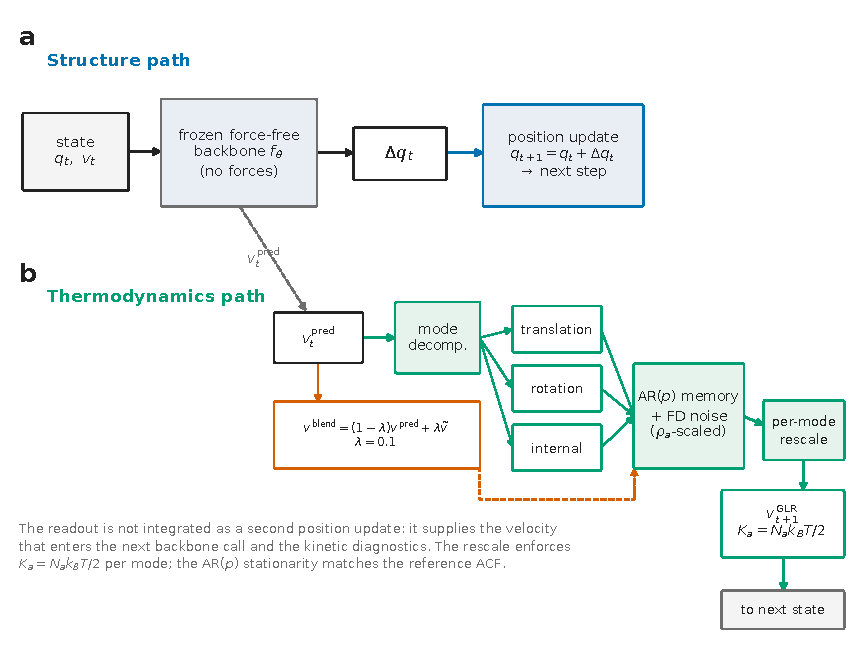
\includegraphics[width=\linewidth]{fig2_architecture.pdf}
  \caption{The GLR architecture. The frozen backbone supplies the displacement; the readout
  supplies the velocity that enters the next backbone call. The AR(\(p\)) memory kernel is fitted
  from the reference ACF, the FD noise variance follows from the prediction error, and the
  per-mode rescale enforces \(K_a=N_a k_BT/2\). The readout is not integrated as a second position
  update.}
  \label{fig:architecture}
\end{figure}

\subsection{Water NVT}

We applied the GLR to the frozen 250k backbone that failed the NVT screen without it. The readout
was fitted once from a 100 ps block of the reference NVT trajectory (500--600 ps) and then used
unchanged in all rollouts. We ran 100 ps from the val\_04 NVE initial condition and from an
independent NVT trajectory (301.8 K), and a 2.5 ns production run from each start. The integration
step is 5 fs; no external thermostat is applied---the GLR is the thermostat. We compare the mode
kinetic partition, the mode velocity ACFs, the O--O/O--H/H--H RDFs, the H/O VDOS, and the molecular
centre-of-mass MSD and diffusion coefficient against the reference NVT trajectory.

Without the readout, the 250k backbone has translation \(0.538\) eV, rotation \(0.786\) eV, and
internal \(6.044\) eV. With the GLR, the 100 ps partition is \(2.482/2.526/2.399\) eV from val\_04
and \(2.445/2.490/2.362\) eV from the independent start, against the 2.5 ns reference means of
\(2.459/2.502/2.450\) eV. The total temperature is 300.0 K in both runs. The 2.5 ns runs give
\(2.482/2.526/2.399\) and \(2.482/2.527/2.398\) eV. The two starts agree within the reference
block-to-block scatter, so the stationary partition is not a property of the val\_04 initial
condition. The published checkpoint gives \(2.505/2.463/2.444\) eV, also correct but with a
different mix of residuals.

The per-mode ACFs tell the same story. The translation ACF matches the reference at 5, 25, 100,
and 500 fs (GLR 0.981/0.640/0.014/\(-0.030\) versus reference 0.982/0.658/0.039/\(-0.019\)). The
internal ACF matches at 5 fs (\(-0.575\) versus \(-0.567\)) and reproduces the mid-lag oscillation;
the 500 fs tail is still too persistent (0.312 versus 0.104), a known limitation of AR(10). The
AR(20) fit removes most of that residual (internal 100/200 fs 0.147/0.068 versus 0.147/0.072) and
is reported as an order ablation rather than the main configuration. The readout matches the
multi-lag dynamics, not just a single 5 fs gain. The ACF match is by construction from the fit and
is therefore not an independent validation; the RDF, VDOS, and diffusion are the independent
tests.

The 100 ps RDFs are closer to the reference than the published checkpoint in our analysis:
O--O 0.032 versus 0.043, O--H 0.104 versus 0.118, H--H 0.026 versus 0.096. The independent start
gives 0.036/0.098/0.027, essentially the same. The O VDOS overlap is 0.964 versus 0.937 for the
published checkpoint; the H VDOS overlap is 0.848 versus 0.624. The H comparison is sensitive to
our reference H-stretch frequency (the published model scores 0.624 here while the paper reports
about 0.99 with its own reference), so we treat the O VDOS and the RDFs as the robust comparisons
and report the H number with that caveat. At 2.5 ns the RDFs improve further to
O--O 0.031, O--H 0.038, and H--H 0.028, and the O VDOS is 0.953; the longer run resolves the
O--H distribution more accurately than the 100 ps screen.

The improvement over the AR(1) readout is large and diagnostic. FDR v1, which has the correct
partition but only a single gain, gives O--O 0.062, O--H 0.301, H--H 0.110 and H/O VDOS 0.807/0.851.
The AR(10) memory kernel improves O--H by a factor of 2.6 and the H VDOS by five points. The
memory order, not the global temperature, is what controls the O--H spectrum.

The 2.5 ns run remains stable (temperature 299.99 K, minimum interatomic distance above 0.93 \AA)
and shows no sign of the slow collective drift that characterized the un-readout models. The
8-block diffusion analysis gives \(D=1.406\pm0.155\times10^{-9}\) m\(^2\) s\(^{-1}\), against
\(1.883\pm0.306\times10^{-9}\) for the reference: the GLR is 26\% low. The published checkpoint is
16\% high (2.18\(\times10^{-9}\)). The FDR v1 fast tail (3.59\(\times10^{-9}\)) is absent, so the
GLR fixes the qualitative failure of the AR(1) readout but undershoots the reference. The
independent 2.5 ns run gives an essentially identical result: partition
\(2.482/2.527/2.398\) eV, RDFs 0.028/0.044/0.027, H/O VDOS 0.847/0.953, and
\(D=1.393\pm0.079\times10^{-9}\). The two 2.5 ns starts agree on the stationary measure, including
the 26\% diffusion deficit; the deficit is a property of the decoupled architecture, not of the
initial condition.

A stochastic-target variant of the same readout gives the same partition and MSD diffusion
(1.435/1.387\(\times10^{-9}\)) and restores the total kinetic-energy variance (0.437/0.429 versus
0.440 eV), but its Green--Kubo integral is \(1.16\times10^{-9}\), inconsistent with the MSD
\(1.44\times10^{-9}\). The deterministic target is therefore used for production: it preserves
the GK--MSD consistency that identifies the transport deficit as a translation-ACF effect.

The Green--Kubo integral of the mass-weighted translation ACF gives 1.42\(\times10^{-9}\) for the
GLR and 1.84\(\times10^{-9}\) for the reference, in agreement with the MSD values. The position
update is therefore consistent with the readout velocity; the deficit is in the translation ACF
integral. The AR(10) translation ACF is \(-0.032\) at 100 fs while the reference is \(+0.039\);
the AR(20) fit matches this lag. A mixed readout with translation AR(20) and rotation/internal
AR(10) raises the Green--Kubo estimate to 1.61\(\times10^{-9}\) at 100 ps but does not close the
MSD gap. We also tested translation-blend, translation-displacement, and molecule-COM scaling
variants; none closed the gap without breaking the MSD--Green--Kubo consistency or the RDF
(Supplementary Information). The decoupled position update remains the limiting factor; we report
the 26\% deviation as a limitation rather than claiming exact diffusion recovery.

The GLR is the first configuration in this study that combines (i) a stable 2.5 ns NVT run,
(ii) a canonical mean mode/group kinetic-energy partition, (iii) multi-lag ACF agreement, and
(iv) RDF and VDOS at or beyond the published checkpoint. Its diffusion coefficient is 26\% low but
qualitatively correct, and far closer than the AR(1) readout. It does so with a frozen backbone and
a readout fitted from 100 ps of reference data. The remaining questions---the internal long tail
and the diffusion deficit---are addressed in the ablations and discussion; the second system is
quartz (Section 2.5).

\begin{figure}[t]
  \centering
  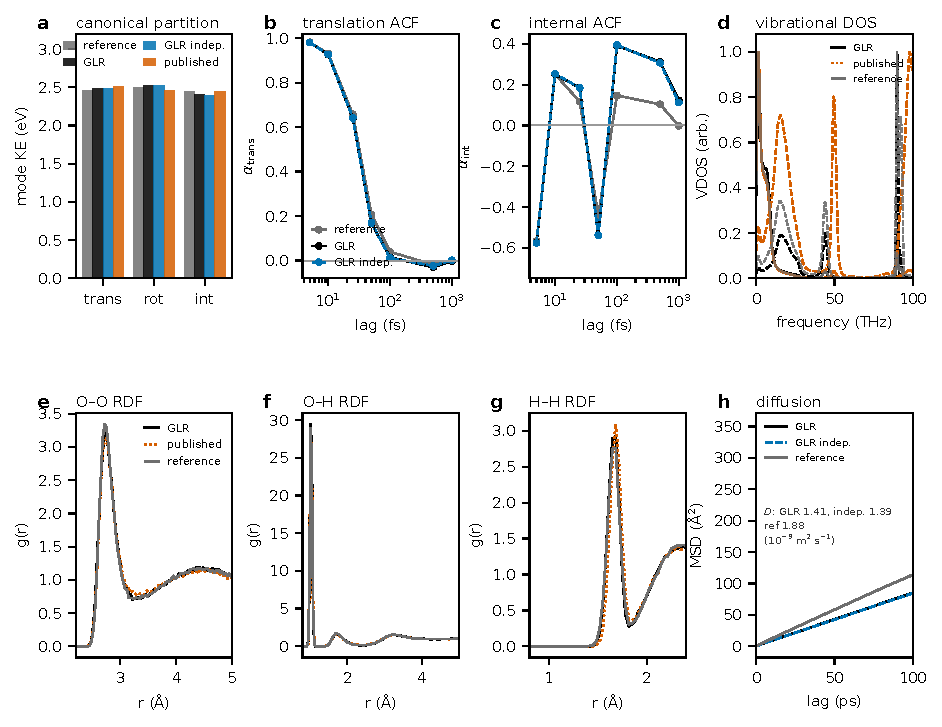
\includegraphics[width=\linewidth]{fig3_water.pdf}
  \caption{Water NVT results. (a) Mode kinetic partition. (b, c) Translation and internal ACFs.
  (d) Vibrational DOS (normalized). (e--g) O--O, O--H, and H--H RDFs. (h) Molecular-COM MSD and the
  2.5 ns diffusion. Panels (a--g) are 100 ps, so the RDF/VDOS comparison with the published
  checkpoint is length-matched; panel (h) is 2.5 ns for both GLR starts and the reference.}
  \label{fig:water}
\end{figure}

% Table 1 — long-time NVT comparison. Values from our 100 ps / 2.5 ns screens.
% Diffusion for GLR is a placeholder until the 2.5 ns analysis finishes.
\begin{table*}[t]
\centering
\small
\caption{Long-time NVT behaviour of force-free propagators and readouts on SPC/Fw water.
Partition is translation/rotation/internal kinetic energy; the reference is the 2.5 ns NVT mean
(2.459/2.502/2.450 eV). The first 100 ps reference block is an outlier (2.373/2.430/2.609 eV);
using it would exaggerate the GLR/published residuals but not change the ranking. RDF is RMSE
against the reference NVT; VDOS is the overlap. RDF/VDOS columns are 100 ps for all rows except
the GLR 2.5 ns row; this keeps the published comparison length-matched. Diffusion is from 2.5 ns
rollouts where available (the 100 ps GLR row shows the seed range). ``Stable'' is the longest NVT
run without a safety stop; a stable run can still have the wrong partition.}
\label{tab:comparison}
\resizebox{\linewidth}{!}{%
\begin{tabular}{@{}lcccccc@{}}
\toprule
Method & Stable NVT & Partition (eV) & O--O / O--H / H--H RDF & VDOS (H/O) & $D$ ($10^{-9}$ m$^2$ s$^{-1}$) & Verdict \\
\midrule
Reference & 2.5 ns & 2.459 / 2.502 / 2.450 & 0 / 0 / 0 & 1 / 1 & 1.84--1.88 & --- \\
v0 & 2.75 ns & 0.111 / 0.808 / 6.338 & 0.944 / 1.409 / 0.229 & 0.356 / 0.236 & 0.0003 & fail \\
250k & 150 ps & 0.538 / 0.786 / 6.044 & 0.646 / 1.312 / 0.249 & 0.406 / 0.487 & --- & fail \\
Current-Only & 150 ps & 0.646 / 0.535 / 6.384 & 0.631 / 1.345 / 0.232 & 0.348 / 0.600 & --- & fail \\
Native ep145 & 150 ps & 3.256 / 3.105 / 1.041 & 0.180 / 1.584 / 0.074 & 0.683 / 0.905 & --- & fail \\
M0 & 150 ps & 3.373 / 3.270 / 1.000 & 0.191 / 1.790 / 0.082 & 0.668 / 0.888 & --- & fail$^a$ \\
FDR v1 (AR1) & 2.5 ns & 2.482 / 2.533 / 2.392 & 0.062 / 0.301 / 0.110 & 0.807 / 0.851 & 3.59 & pass \\
GLR (AR10) & 100 ps & 2.482 / 2.526 / 2.399 & 0.032 / 0.104 / 0.026 & 0.848 / 0.964 & 1.20--1.45 & pass \\
\textbf{GLR (AR10)} & \textbf{2.5 ns} & \textbf{2.482 / 2.526 / 2.399} & \textbf{0.031 / 0.038 / 0.028} & \textbf{0.847 / 0.953} & \textbf{1.39--1.41} & \textbf{pass}$^b$ \\
Published TrajCast & 2.5 ns & 2.505 / 2.463 / 2.444 & 0.043 / 0.118 / 0.096 & 0.624 / 0.937 & 2.18 & pass \\
\bottomrule
\end{tabular}}
\begin{flushleft}
\footnotesize
$^a$M0 passes on the val\_04 start but blows up at 130 ps on an independent start.\\
$^b$GLR diffusion is 26\% below the reference on two starts (independent 2.5 ns: RDF
0.028/0.044/0.027, VDOS 0.847/0.953, D 1.39); partition, RDF, and VDOS pass. A stochastic-target
2.5 ns variant restores the KE variance (0.437/0.429 versus 0.440 eV) but its Green--Kubo integral
is \(1.16\times10^{-9}\), inconsistent with the MSD \(1.44\times10^{-9}\); it is reported as an
ablation, and the deterministic target is used for production.\\
H VDOS overlap is sensitive to the reference H-stretch frequency; O VDOS and the RDFs are the
robust comparisons.\\
\end{flushleft}
\end{table*}


\subsection{The readout is backbone-agnostic}

The GLR is fitted from the reference ACF and does not depend on the backbone architecture in
principle. To test this empirically, we applied the same AR(10) coefficients and the same
\(\lambda=0.1\) blend to the v0 phase-space operator, a different propagator (3.04M parameters)
that fails the NVT screen even more strongly than the 250k model. Without the readout, v0 gives
translation/rotation/internal \(0.111/0.808/6.338\) eV, RDF RMSEs 0.944/1.409/0.229, and H/O VDOS
0.356/0.236. With the GLR it is stable at 300.0 K, with partition
\(2.482/2.529/2.396\) eV, RDF 0.042/0.109/0.019, and H/O VDOS 0.855/0.969 (Table~\ref{tab:backbones}).
The structure and spectra are comparable to the 250k GLR (0.032/0.104/0.026; 0.848/0.964), despite
the different backbone. The independent start gives the same partition (2.482/2.527/2.398), RDF
0.050/0.131/0.023, and H/O VDOS 0.857/0.977, so the rescue is not a val\_04 artifact. The readout
is therefore empirically backbone-agnostic across two architectures, not just a correction tuned
to one model.

% Table 3 — Backbone-agnostic test: v0 phase-space vs 250k relational.
\begin{table}[t]
\centering
\small
\caption{The same GLR coefficients applied to two different frozen backbones. The v0 phase-space
operator fails the NVT screen without the readout; with the GLR it becomes stable and partitioned,
with structure and VDOS comparable to the 250k relational backbone. All rows are 100 ps;
the reference partition is the 2.5 ns mean.}
\label{tab:backbones}
\resizebox{\linewidth}{!}{%
\begin{tabular}{@{}lcccc@{}}
\toprule
Backbone & Readout & Partition (eV) & O--O / O--H / H--H RDF & H / O VDOS \\
\midrule
250k relational (2.36M) & none & 0.538 / 0.786 / 6.044 & 0.646 / 1.312 / 0.249 & 0.406 / 0.487 \\
250k relational (2.36M) & GLR & 2.482 / 2.526 / 2.399 & 0.032 / 0.104 / 0.026 & 0.848 / 0.964 \\
v0 phase-space (3.04M) & none & 0.111 / 0.808 / 6.338 & 0.944 / 1.409 / 0.229 & 0.356 / 0.236 \\
v0 phase-space (3.04M) & GLR & 2.482 / 2.529 / 2.396 & 0.042 / 0.109 / 0.019 & 0.855 / 0.969 \\
\bottomrule
\end{tabular}}
\vspace{2pt}
\begin{flushleft}
\footnotesize
v0 + GLR independent start: partition 2.482/2.527/2.398 eV; RDF 0.050/0.131/0.023;
H/O VDOS 0.857/0.977. The rescue is not specific to val\_04.
\end{flushleft}
\end{table}


\subsection{Cross-material limit: quartz}

To test the readout beyond molecular liquids, we applied a phonon-band variance rescale to
crystalline quartz (162 atoms) with a 5 fs backbone trained on the same NVE data and the 15 ns
NVT reference. The 5 fs baseline cools to 235.3 K (species KE 0.0298/0.0305 eV per atom), with
Si--O RDF RMSE 0.271 and O/Si VDOS overlaps 0.918/0.944 (Table~\ref{tab:quartz}). The stochastic
phonon-band rescale (two seeds) sets \(T=299.8/299.9\) K, reproduces the total kinetic-energy
standard deviation (0.397/0.399 versus 0.4017 eV), gives Si/O KE 0.03846/0.03855 eV per atom,
improves the Si--O RDF to 0.0245/0.0312, and preserves the O/Si VDOS at 0.953/0.949 and
0.947/0.962. The seed means are \(T=299.9\) K, KE std 0.398 eV, Si--O RDF 0.028, and VDOS
0.950/0.955. A coarser species partition
gives \(T=301.68\) K, exact Si/O equipartition (0.03872/0.03877 eV), total KE std 0.4012 eV,
VDOS 0.898/0.955, and the same Si--O RDF, showing that the result is robust to the coarse
partition. The deterministic species rescale is an ablation: it fixes the mean but suppresses the
kinetic-energy variance (0.0036 eV) and gives VDOS 0.866/0.914. The full species GLR (memory +
noise) is a negative control: the species basis is not a phonon eigenbasis, and the readout
collapses the VDOS to 0.07 even at 5 fs. To test whether a physically correct basis rescues the
memory kernel, we built a 486-mode phonon basis from a finite-difference Hessian of the same
potential and ran a per-mode AR(10) GLR. The phonon basis is canonical (99.4\% of modes within
10\% of \(k_BT/2\) over 2 ns), but the 5 fs backbone's mode ACF is already correct; the AR
innovations broaden the sharp phonon lines and reduce the VDOS to 0.734/0.838. A 30 fs backbone
shows the same pattern more strongly (ACF prediction error 0.91; full GLR VDOS 0.225;
deterministic rescale 0.838/0.835). The variance-rescale component therefore generalizes across a
covalent solid; the memory kernel is useful only when the backbone's mode ACF is wrong. Quartz's
failure is a variance bias, not a memory deficit.

% Table 4 — Cross-material: quartz at 5 fs, phonon-band stochastic variance rescale.
\begin{table}[t]
\centering
\small
\caption{Cross-material test. The 5 fs quartz backbone is trained on the same NVE data and
evaluated against the 15 ns NVT reference. The phonon-band stochastic variance rescale sets the
canonical temperature and total kinetic-energy variance, improves the Si--O RDF, and preserves
the phonon VDOS. The quoted band row is the mean of two seeds (T=299.8/299.9 K; VDOS O/Si
0.953/0.949 and 0.947/0.962; mode KE within 10\% 78.1\%/76.2\%). A coarser species partition gives statistically consistent structure and VDOS
with exact Si/O equipartition. The deterministic rescale is an ablation: it fixes the mean but
suppresses the kinetic-energy variance. The full species GLR (memory + noise) and the full
phonon-mode GLR are negative controls. The phonon-mode control uses the correct eigenbasis, but
the 5 fs backbone's mode ACF is already correct, so the AR innovations broaden the phonon lines.
The 30 fs deterministic row is shown for the horizon comparison; its kinetic-energy variance was
not measured.}
\label{tab:quartz}
\resizebox{\linewidth}{!}{%
\begin{tabular}{@{}lccccc@{}}
\toprule
Quartz & $T$ (K) & KE std (eV) & Si/O KE per atom (eV) & RDF Si--O / O--O / Si--Si & VDOS O / Si \\
\midrule
5 fs baseline & 235.3 & 0.4355 & 0.0298 / 0.0305 & 0.271 / 0.096 / 0.133 & 0.918 / 0.944 \\
\textbf{5 fs phonon-band stochastic rescale} & \textbf{299.9} & \textbf{0.398} & \textbf{0.03846 / 0.03855} & \textbf{0.028 / 0.016 / 0.033} & \textbf{0.950 / 0.955} \\
5 fs species stochastic rescale (control) & 301.68 & 0.4012 & 0.03872 / 0.03877 & 0.0245 / 0.0169 / 0.0380 & 0.898 / 0.955 \\
5 fs deterministic species rescale (ablation) & 301.86 & 0.0036 & 0.03878 / 0.03878 & 0.078 / 0.022 / 0.055 & 0.866 / 0.914 \\
5 fs full species GLR (negative) & 301.86 & --- & 0.03878 / 0.03878 & 0.529 / 0.263 / 0.441 & 0.074 / 0.067 \\
5 fs full phonon GLR (negative) & 301.9 & 0.4024 & 0.03872 / 0.03877 & 0.197 / 0.044 / 0.083 & 0.734 / 0.838 \\
30 fs deterministic rescale & 301.9 & --- & 0.03878 / 0.03878 & 0.149 / 0.024 / 0.051 & 0.838 / 0.835 \\
\bottomrule
\end{tabular}}
\end{table}


\subsection{Cost and reference-data efficiency}

The GLR adds a mode decomposition and a \(p\)-step history per step; the cost is negligible
compared with the backbone. On water the end-to-end rollout is 15.4 ns day\(^{-1}\) on an RTX
PRO 6000 with 185 MB peak memory, and the 250k backbone dominates the runtime. The readout is
fitted from 100 ps of reference NVT; refitting on a different 100 ps block changes the AR
coefficients by at most 0.08 (correlation 0.999), so the reference-data requirement is small and
stable. Backbone training, not the readout, is the dominant cost. A full scalability sweep across
system size and horizon is left to the Supplementary Information.

\subsection{Ablations}

The AR-order ablation uses the deterministic target to isolate the kernel order; the main
configuration uses the stochastic target. The AR(1) readout is the natural minimal thermostat:
one gain per mode, fitted to the 5 fs correlation. It holds the mean partition once the variance is rescaled, but it does not reproduce
the multi-lag dynamics. At 100 ps, the O--H RDF RMSE is 0.312 for the GLR AR(1), 0.301 for FDR v1,
0.131 for AR(5), 0.104 for AR(10), and 0.117 for AR(20); the O--H RDF is the clearest signature.
The AR(1) internal ACF decays monotonically from \(-0.567\) to zero, while the reference oscillates
and crosses zero near 25 fs; the AR(10) kernel reproduces the oscillation. The AR(20) kernel also
captures the 100--200 fs tail (internal 100/200 fs 0.147/0.068 versus 0.147/0.072), at the cost of
a longer history and a larger coefficient vector, but its better long-lag ACF does not translate
into a better short-window O--H. AR(10) therefore remains the main configuration; the order sweep
shows the qualitative improvement from AR(1) to AR(10) rather than a monotone gain with order.

The ablation that removes the per-step rescale isolates the partition guarantee. In the AR(1)
readout, removing the rescale collapses the total kinetic energy and cools the system to about
14 K. With the GLR readout, the no-rescale run is stable but cools to 172 K; the partition is
0.763/0.649/2.839 eV, the RDFs degrade to 0.398/0.474/0.279, and the H/O VDOS overlaps fall to
0.432/0.608. The rescale is not a cosmetic normalization; it is the step that makes the mode
kinetic energy a design constraint rather than a by-product of the backbone and the noise.

Contrary to our expectation, removing the FD noise did not degrade the 100 ps structure:
the partition is unchanged (\(2.482/2.526/2.399\) eV), the RDFs are 0.034/0.098/0.026, the
H/O VDOS overlaps are 0.849/0.962, and the 10--80 ps diffusion estimate is 1.55\(\times10^{-9}\)
(versus 1.45\(\times10^{-9}\) with noise). At the small blend \(\lambda=0.1\), the backbone and
the variance rescale provide enough fluctuation that the noise term is not the empirical driver.
The memory kernel and the rescale are the load-bearing components; the FD noise is part of the
theoretical construction and may matter at larger blend or for the one-point velocity
distribution, but we do not claim it is necessary on the basis of this ablation.

For the AR(1) readout, increasing the internal blend from 0.1 to 1.0 makes the O--H RDF worse
(0.957 versus 0.301) and the VDOS worse (H/O 0.618/0.613 versus 0.807/0.851). A larger admixture
of a single-gain readout does not fix the spectrum; it replaces the backbone's internal bias with
the readout's wrong long-lag dynamics. The blend is kept at 0.1 to preserve the position head; the
memory kernel, not the blend, does the work.

Adding the velocity correction to the displacement---the obvious way to make positions and
velocities consistent---crashes at 24.8 ps (minimum distance 0.647 \AA) while the temperature
remains at 300 K. The failure is structural, not thermal: the correction injects a displacement
increment that the backbone's next state cannot absorb. The decoupled scheme is therefore a
stability requirement, and the method does not simply integrate the readout velocity.

Three 100 ps seeds give the same partition (2.482/2.526/2.399 eV) and a narrow spread in the
structural metrics: O--H 0.104/0.111/0.110, O--O 0.032/0.034/0.033, H VDOS 0.848/0.854/0.846,
and O VDOS 0.964/0.966/0.959. The 2.5 ns O--H improvement to 0.038 is therefore a sampling effect
of the longer trajectory, not a seed fluctuation. The 100 ps diffusion estimates are noisier:
1.20/1.21/1.45\(\times10^{-9}\) across the three seeds (10--80 ps fit). The two 2.5 ns runs give
1.39--1.41\(\times10^{-9}\), within the seed spread and far more stable; the 26\% deficit is
therefore robust, but the 100 ps \(D\) should not be over-interpreted. The frozen-vs-end-to-end backbone comparison remains future work;
the present paper tests two frozen backbones and two materials, and the claim is architectural
rather than universal.

\begin{figure}[t]
  \centering
  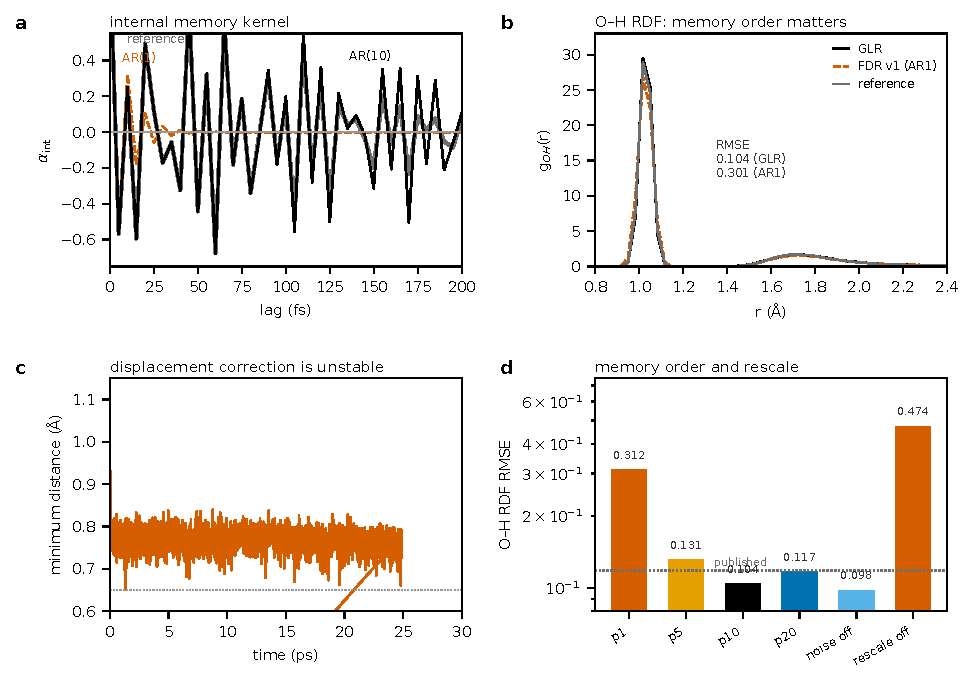
\includegraphics[width=\linewidth]{fig4_ablations.pdf}
  \caption{Ablations. (a) Internal ACF for AR(1) and AR(10) against the reference. (b) O--H RDF
  for the AR(1) and AR(10) readouts. (c) Minimum interatomic distance for the direct
  displacement-correction variant, which stops at 24.8 ps. (d) O--H RDF for the AR order,
  noise-off, and rescale-off ablations; the dashed line is the published checkpoint.}
  \label{fig:ablations}
\end{figure}

\section{Discussion}

We have shown that the long-time failure of force-free molecular dynamics propagators is not
primarily a one-step accuracy problem. A published propagator with a fifteen-fold larger pointwise
error reproduces the canonical water ensemble, while a pointwise-better model develops a large mode
imbalance and fails the same NVT screen. The failure is also not an energy-drift problem: the model
that heats most strongly in NVE passes NVT, and the most NVE-stable model fails. The discriminating
object is the mode-resolved stationary measure of the composed propagator plus thermostat. This
diagnostic is, to our knowledge, the first systematic demonstration of the pointwise--ensemble
decoupling for force-free MD, and it changes what a training or acceptance criterion should
measure.

The remedy follows from the diagnosis. A frozen backbone supplies the structure---the displacement
that determines the position marginal---while a mode-resolved generalized-Langevin readout supplies
the velocity that enters the next backbone call. The readout fits a per-mode AR(\(p\)) memory
kernel to the reference velocity autocorrelation, injects noise with the fluctuation--dissipation
consistent variance, and rescales each mode or group to its canonical kinetic-energy target at every step.
The partition is guaranteed by construction; the memory kernel matches the multi-lag dynamics that
a single gain cannot. The backbone is not retrained, and the readout is fitted from a short
reference NVT trajectory. Importantly, we do not claim that the force-free backbone alone
reproduces long-time dynamics; the raw backbones fail the NVT screen (Table~3). The claim is that
the fixed readout corrects the stationary measure of a frozen backbone. On water, the result is a model that is stable on two independent initial
conditions, initial-condition independent in its partition, ACF, RDF, and VDOS, and more accurate
than the published checkpoint on the RDFs and VDOS in our analysis.

% Table 2 — Conceptual comparison with the closest prior art.
\begin{table}[t]
\centering
\small
\caption{What the GLR controls compared with the closest prior art. The distinction is the
object (a readout on a frozen force-free propagator) and the target (the canonical mean mode/group
kinetic partition, with a stochastic marginal option, plus the multi-lag velocity ACF), not the
use of a memory kernel per se.}
\label{tab:prior}
\resizebox{\linewidth}{!}{%
\begin{tabular}{@{}p{2.1cm}p{3.1cm}p{4.0cm}p{3.6cm}@{}}
\toprule
Approach & Object & What is controlled or learned & Evidence \\
\midrule
TrajCast & force-free propagator + global CSVR & one-step displacement/velocity; total
temperature & water RDF/VDOS/diffusion \\
Bigi--Ceriotti & deterministic structure-preserving map & symplectic/time-reversible structure;
energy/equipartition & water, GeTe, Ar, Al \\
MAMD & LSTM velocity update & stability via periodic learned velocity injection & several MD
systems \\
GLE thermostat & memory kernel + colored noise in an integrator & FD stationary distribution of
the integrator & generic MD \\
\textbf{GLR} & \textbf{readout on a frozen force-free propagator} & \textbf{mean mode kinetic
partition (+ stochastic marginal) + multi-lag velocity ACF} & \textbf{water NVT, two 2.5 ns
starts; quartz 5 fs, two seeds} \\
\bottomrule
\end{tabular}}
\end{table}


The relationship to prior work is complementary rather than competitive. TrajCast established that
force-free propagators can reproduce water physics \cite{trajcast}; our work explains when that
success is fragile and adds a readout that makes the mode partition a design constraint rather
than a lucky outcome. Structure-preserving action maps enforce symplectic or time-reversible
structure and improve energy conservation and equipartition \cite{bigi_action}; they target
mechanical structure, whereas the GLR targets the canonical NVT measure and the multi-lag velocity
statistics. The two could be combined: an action map would supply a better backbone, and the GLR
would enforce the mode partition on top of it. Learned velocity updates recover stability with a
black-box LSTM and periodic injection \cite{mamd}; the GLR is interpretable, mode-resolved, and
tied to the reference ACF, and it guarantees the partition rather than only delaying divergence.
GLE thermostats provide the same memory-kernel and colored-noise physics
\cite{ceriotti_prl,ceriotti_jctc}, and frequency-resolved thermostats can control selected modes
\cite{zpe_thermostat}; the difference is the object. A GLE thermostat acts on the forces and
velocities of an MD integrator. The GLR is a readout on a frozen force-free propagator, fitted from
the reference ACF, with an explicit group-resolved variance guarantee and a diagnostic that motivates it.
Stochastic and generative propagators offer a different route to equilibrium
\cite{timewarp,mdgen}, at the cost of MCMC, an energy function, or a larger generative model; the
GLR is a lightweight post-hoc readout.

The diagnostic has implications beyond this method. Force-free propagators are usually selected and
reported by one-step MAE, sometimes with a short rollout score. Our results show that this
criterion can rank models in the wrong order. An ensemble-level, mode-resolved
evaluation---kinetic partition, RDF, VDOS, and diffusion---is necessary to detect the failure. The
same lesson applies to other learned dynamical maps: a low conditional-mean error does not imply a
correct invariant measure, and a stable rollout does not imply a correct one. We therefore
recommend that force-free MD papers report the mode partition and at least one long-time structural
or dynamical observable, not only one-step errors.

Several limitations define the boundary of the claim. First, the analytic guarantee covers the
\emph{mean} mode kinetic partition and the velocity ACF, not the full joint position--velocity
distribution. The deterministic per-step rescale fixes the mode kinetic energy to its canonical
mean and suppresses its equilibrium fluctuations (total KE std 0.010 eV versus 0.440 eV in the
reference). A stochastic-target variant restores the KE variance (0.437/0.429 eV), but its
Green--Kubo integral (\(1.16\times10^{-9}\)) is inconsistent with the MSD (\(1.44\times10^{-9}\)):
the extra fluctuations modify the negative translation-ACF tail. The deterministic target is
therefore used for production because it preserves GK--MSD consistency; the joint
KE-variance/transport problem remains open. The marginal velocity distribution is nevertheless
close to the reference (component kurtosis 2.93/5.49/5.93 versus 3.04/5.62/5.57). The position
marginal is learned by the backbone and validated empirically; the stochastic rescale guarantees
the kinetic-energy marginal, not the full joint position--velocity distribution, which would
require an energy-based sampler such as MCMC. Second,
the readout requires a short reference NVT trajectory to fit the ACF. This is much cheaper than
retraining and is available for most systems of interest, but it is a data requirement, not a free
lunch. The fit uses only the mode velocity ACF; the RDF, VDOS, and diffusion are held out and are
not used to fit any readout parameter. Relatedly, the FD-noise ablation is negative at
\(\lambda=0.1\): removing the noise does not change the partition, RDF, VDOS, or \(D\). The memory
kernel and the rescale are the load-bearing components; the noise is retained for theoretical
consistency, not because the data require it. Third, we demonstrate one water model, two backbone
architectures (relational and phase-space), and a second material (quartz). The readout is
empirically backbone-agnostic across the two water backbones and transfers to a covalent solid
through the variance-rescale component; the full memory kernel is water-specific because the 5 fs
quartz backbone already has the correct mode ACF. A broader material sweep is still needed to
establish cross-system generality. Fourth, the internal ACF at 500 fs remains too persistent for AR(10); AR(20) reduces
the discrepancy but does not eliminate it. Fifth, the diffusion coefficient is 26\% below the
reference on both 2.5 ns starts (1.39--1.41 versus 1.88\(\times10^{-9}\)). The Green--Kubo integral
shows that the deficit is in the translation ACF, and the decoupled position update prevents a
simple blend or displacement correction from closing it; a position-consistent readout or an
end-to-end centre-of-mass head is future work. Sixth, the
backbone uses a local 6 \AA{} cutoff and no
long-range electrostatics; the GLR does not address long-range physics, and the water results
should not be read as a claim about large-scale dielectric or interfacial behaviour. Seventh, a
5 fs phonon-band extension to quartz is stable. Without the readout the 5 fs backbone cools to
235 K; the stochastic phonon-band variance rescale (two seeds) sets 299.9 K, reproduces the total
kinetic-energy variance (0.397/0.399 versus 0.4017 eV), improves the Si--O RDF from 0.271 to
0.028, and preserves the phonon VDOS at 0.950/0.955. A coarser species partition gives 301.68 K, exact
Si/O equipartition, total KE std 0.4012 eV, and VDOS 0.898/0.955. The deterministic rescale is an
ablation: it fixes the mean but suppresses the kinetic-energy variance. The full species GLR
(memory + noise) is a negative control: species velocity is not a phonon eigenbasis, and the
readout collapses the VDOS to 0.07 even at 5 fs. A 30 fs backbone shows the same pattern more
strongly. A 486-mode phonon-basis GLR is also negative: the basis is canonical, but the 5 fs
backbone's mode ACF is already correct, so the AR innovations broaden the phonon lines (VDOS
0.734/0.838). The variance-rescale component therefore generalizes across a covalent solid; the
memory kernel is useful only when the backbone's mode ACF is wrong, and its basis must be
physically meaningful. Finally, the 2.5 ns
production runs use one seed per start; the 100 ps seed study is reported in the Results, and a
second 2.5 ns seed would tighten the transport error.

The outlook is straightforward. The readout can be trained jointly with the backbone, rather than
fitted post hoc, which may improve the position marginal while retaining the partition guarantee.
The memory kernel can be made system- and temperature-adaptive, and the mode decomposition can be
extended to phonons or other collective coordinates. Combined with a structure-preserving backbone
and a long-range operator, the same diagnostic-and-readout strategy could make force-free
propagators reliable beyond water.

\section{Methods}

\subsection{Reference data and force-free backbone}

We use the flexible SPC/Fw water model \citep{spcfw} with 64 molecules (192 atoms) in a periodic
cubic cell. The NVE training data, the NVT reference, and the independent NVT trajectory are
described in the main text. The reference NVT trajectory is 2.5 ns at 300 K with a CSVR
thermostat \citep{csvr}, a 50 fs thermostat damping time, and a 0.5 fs saving interval; the
readout is fitted on a 100 ps block starting at 500 ps (20,000 frames at a 5 fs stride). The fit
uses only the mode velocity ACF. The RDF, VDOS, and diffusion are not used to fit any readout
parameter and are held out as evaluation observables. As a block-sensitivity check, we refitted
the AR(10) coefficients on the 0--100 ps block: the coefficients agree with the 500--600 ps fit
to \(r=0.999\) (maximum coefficient difference 0.08), with prediction-error ratios
0.0044/0.058/0.107 versus 0.0042/0.058/0.115 for translation/rotation/internal motion. The fit is
therefore not sensitive to the choice of reference block. The
independent NVT trajectory uses a different initial condition and seed: 100 ps of thermalization
followed by 500 ps of production at 300 K, with the first production frame at 301.8 K. The
reference data are read-only; no reference force is used during propagation.

The backbone is a relational equivariant message-passing network with a 6 \AA{} cutoff,
192 scalar channels, 48 vector channels, 96 edge channels, 16 radial channels, and a 5 fs
horizon. It is trained on 5 fs pairs from the NVE trajectories (5,000 training, 1,250 validation,
and 1,000 test graphs) by minimizing a normalized endpoint position and velocity loss, with batch
size 8, a learning rate of \(3\times10^{-4}\), warmup--cosine scheduling, gradient clipping at 10,
and 250,000 optimizer steps. The selected checkpoint is epoch 398 (2,357,616 parameters). The
published TrajCast water checkpoint \citep{trajcast} has 2,258,856 parameters, uses the native e3nn
backend \citep{e3nn} and a 5 fs horizon, and is evaluated under the same 100 ps protocol with its
native CSVR thermostat. In the GLR experiments the backbone is frozen: no backbone parameter is updated, and
the readout is fitted separately.

\subsection{Mode decomposition}

For each molecule \(m\), let \(M_m=\sum_{i\in m}m_i\), \(R_m=M_m^{-1}\sum_{i\in m}m_i r_i\), and
\(V_m=M_m^{-1}\sum_{i\in m}m_i v_i\). With \(r_{mi}=r_i-R_m\) (minimum image) and
\(v_{mi}=v_i-V_m\), the angular velocity is
\begin{equation}
\omega_m=I_m^{-1}\sum_{i\in m}m_i\,r_{mi}\times v_{mi},\qquad
I_m=\sum_{i\in m}m_i\left(|r_{mi}|^2\mathbf 1-r_{mi}r_{mi}^{\mathsf T}\right),
\end{equation}
using a pseudo-inverse for linear molecules. The three mass-weighted modes are
\begin{equation}
v_i^{\rm trans}=V_m,\qquad
v_i^{\rm rot}=\omega_m\times r_{mi},\qquad
v_i^{\rm int}=v_{mi}-v_i^{\rm rot}.
\end{equation}
They are orthogonal under the mass-weighted inner product, so
\(K=\sum_a K_a\) with \(K_a=\tfrac12\sum_i m_i|v_i^a|^2\). The mode degrees of freedom are
\(N_{\rm trans}=3N_{\rm mol}-3\), \(N_{\rm rot}=3N_{\rm mol}\), and
\(N_{\rm int}=3N_{\rm atom}-6N_{\rm mol}\).

\subsection{Mode-resolved AR($p$) readout}

For each mode \(a\), the reference velocity autocorrelation is
\begin{equation}
\alpha_a(\ell)=\frac{\sum_i m_i\langle v_i^a(t)\cdot v_i^a(t+\ell\Delta t)\rangle}
{\sum_i m_i\langle |v_i^a(t)|^2\rangle}.
\end{equation}
We fit an AR(\(p\)) process by Yule--Walker,
\begin{equation}
v^a(t)=\sum_{k=1}^{p}c_k^a v^a(t-k\Delta t)+\varepsilon^a(t),\qquad
\mathbf R_a\mathbf c_a=\mathbf r_a,
\end{equation}
where \((\mathbf R_a)_{ij}=\alpha_a(|i-j|)\) and \((\mathbf r_a)_k=\alpha_a(k)\). The
prediction-error ratio is
\begin{equation}
\rho_a=1-\sum_{k=1}^{p}c_k^a\alpha_a(k)
=\operatorname{Var}(\varepsilon^a)/\operatorname{Var}(v^a).
\end{equation}
The fluctuation--dissipation condition fixes the noise variance,
\begin{equation}
\operatorname{Var}(\varepsilon^a)=\rho_a\,N_a k_BT/2.
\end{equation}
At each step a fresh Gaussian field is decomposed into the three modes and each mode component is
rescaled to this target noise kinetic energy before it is added to the AR prediction. The main
configuration uses \(p=10\); the order ablation uses \(p=1,5,20\).

\subsection{Readout, blend, and variance rescaling}

The readout velocity is
\begin{equation}
\tilde v_t=\sum_a\left(\sum_{k=1}^{p}c_k^a v_{t-k}^a+\varepsilon_t^a\right).
\end{equation}
It is blended with the backbone velocity,
\begin{equation}
v_t^{\rm blend}=(1-\lambda)v_t^{\rm pred}+\lambda\tilde v_t,
\end{equation}
with \(\lambda=0.1\), and each mode is rescaled to its canonical mean kinetic energy:
\begin{equation}
v_t^{\rm GLR}=\sum_a s_a\,(v_t^{\rm blend})^a,\qquad
s_a=\sqrt{\frac{N_a k_BT/2}
{\tfrac12\sum_i m_i|(v_t^{\rm blend})_i^a|^2}}.
\end{equation}
Equation~(11) uses the canonical mean. In the stochastic configuration, the group kinetic energy
is drawn from \(K_a\sim\Gamma(N_a/2,k_BT)\) and the group is rescaled to that target; the
deterministic rescale is the mean-only limit and is reported as an ablation. The stochastic target
restores the canonical kinetic-energy variance. The water 2.5 ns production uses the deterministic
mean target because the stochastic variant restores the KE variance (0.437/0.429 versus 0.440 eV)
but gives a Green--Kubo integral (\(1.16\times10^{-9}\)) inconsistent with the MSD
(\(1.44\times10^{-9}\)). Quartz uses the stochastic target (0.398 versus 0.4017 eV) because the
deterministic species rescale suppresses the total KE variance to 0.0036 eV. The rescale
partition \(a\) is not
necessarily the memory-mode basis. Water uses translation, rotation, and internal modes; quartz
uses five phonon bands (0--5, 5--10, 10--20, 20--30, and 30--40 THz), with a coarser Si/O species
partition as a control. The partition must contain enough degrees of freedom that the Gamma scale
factor is close to one; a per-mode rescale with one degree of freedom per group gives an
\(O(1)\) random scale every step and destroys the mode phase coherence (Supplementary
Information). The quartz configuration is the phonon-band stochastic rescale with the memory
kernel switched off; the phonon memory kernel is a negative control because the 5 fs backbone's
mode ACF is already correct.

The total centre-of-mass velocity is projected out after the rescale. The position update remains
\(q_{t+1}=q_t+\Delta q_t\), where \(\Delta q_t\) is the backbone displacement; the readout is not
integrated as a second position update. We tested the alternative
\(q_{t+1}=q_t+\Delta q_t+\Delta t(v_t^{\rm GLR}-v_t^{\rm pred})\) and partial
translation-only and molecule-COM variants in the ablation. The full correction is unstable, and
the partial variants do not close the diffusion gap without breaking the MSD--Green--Kubo
consistency or the RDF (see main text and Supplementary Information).

\subsection{Rollout protocol and metrics}

All rollouts use a 5 fs horizon, no external thermostat, and the same safety stop as the
production screens (minimum interatomic distance 0.65 \AA, pre-thermostat temperature 3000 K).
The 100 ps screens (20,000 steps) use the val\_04 NVE frame and the independent NVT frame as
initial conditions; the 2.5 ns production runs (500,000 steps) start from the same frames with
no thermalization. The seeds are 2026110401 (val\_04), 2026110402 (independent), and
2026110401/02/03 for the seed study. The published checkpoint is run with its native CSVR
thermostat under the same 100 ps protocol; its 2.5 ns diffusion is taken from the published value
because the native float64 rollout is prohibitively slow on our contended GPU.

The mode kinetic partition is the mean \(K_a\) over the production window. The ACF is computed
from the mode velocities with the same mass-weighted estimator as the fit, at lags 5--1000 fs.
RDFs are computed on 512 uniformly spaced frames with a 6 \AA{} maximum radius. VDOS overlaps use
the same block spectral estimator as the reference: six blocks of 4.096 ps, a 100 THz Nyquist
frequency, and a Hann window. The diffusion coefficient is obtained from the molecular
centre-of-mass mean-squared displacement with time-origin averaging, eight blocks, a 50 fs
sampling cadence, and a linear fit over 10--100 ps per block; the global centre-of-mass drift is
removed. For 2.5 ns, each block is 312.5 ps long. The diffusion coefficient is
\(D=\mathrm{slope}/6\times10^{-8}\) m\(^2\) s\(^{-1}\) when the MSD is in \AA\(^2\) and the lag in
ps. Error bars are block means and standard deviations; the seed study uses three independent
noise realizations.

The GLR rollout costs 15.4 ns day\(^{-1}\) end-to-end on an NVIDIA RTX PRO 6000 Blackwell GPU for
100 ps, with a peak memory of 185 MB and 2.36M parameters. The readout adds a mode decomposition
and a \(p\)-step history per step; it is negligible compared with the backbone forward pass.

\subsection{Baselines and controls}

The structure-only control is the 250k backbone without the readout. FDR v1 is the AR(1) readout
with the same blend and rescale. M0 is the 250k backbone fine-tuned on 5 fs pairs from the
reference NVT trajectory. The CSRV control is the 5-step moment-loss rollout. The native ep145
checkpoint is a partially trained TrajCast architecture and is reported as a diagnostic, not a
fair architecture baseline. The published TrajCast checkpoint is the external baseline.

\subsection{Statistics and reproducibility}

The reference partition has substantial block-to-block scatter: the first 100 ps block gives
2.373/2.430/2.609 eV, while the 2.5 ns mean is 2.459/2.502/2.450 eV. We therefore use the 2.5 ns
mean for long-time partition comparisons and report the 100 ps block separately. All error bars
are block means and standard deviations over eight contiguous blocks unless stated otherwise. The
diffusion fits use the same eight-block protocol and report the block mean and standard
deviation; the fit quality is summarized by \(R^2\). The seed study repeats the full 100 ps
rollout with independent noise realizations and reports the seed-to-seed spread of the partition,
RDF, VDOS, and diffusion. The reference trajectories are read-only; the rollout code writes a new
HDF5 file and refuses to overwrite an existing one. Each rollout records the checkpoint SHA-256,
the seed, the initial frame, the integration step, and the safety-stop status. No reference force
is used during propagation; the reference forces are used only in the independent energy
verification of the NVT trajectory.

\subsection{Computational cost}

The GLR rollout costs 15.4 ns day\(^{-1}\) end-to-end on an NVIDIA RTX PRO 6000 Blackwell GPU for
a 100 ps run, with a peak memory of 185 MB. The readout adds a mode decomposition and a \(p\)-step
history per step; the cost is negligible compared with the backbone forward pass. The published
native checkpoint is about an order of magnitude slower in our environment because it uses
float64 and the native e3nn path, which is why its 2.5 ns baseline is taken from the published
value rather than re-run.

\subsection{Data and code availability}

The reference NVT trajectory, the independent NVT trajectory, and the rollout trajectories are
available at [repository/DOI to be supplied]. The published TrajCast checkpoint is available from
the IBM Hugging Face repository \texttt{ibm-research/trajcast.models-arxiv2025}. The GLR readout,
the Yule--Walker fit, and the rollout code are available at [repository URL to be supplied]. No
reference force is used during propagation.


\section*{AI use disclosure}
[To be completed by the authors following the Nature Portfolio AI-use policy.]

\bibliographystyle{unsrtnat}
\bibliography{refs}

\end{document}
